
\documentclass{beamer}
\usepackage[latin1]{inputenc}
%\usetheme{Montpellier}
%\usetheme{Boadilla}
%\usecolortheme[RGB={204,51,255}]{structure}
%\usecolortheme[named=purple]{structure}
\usecolortheme[RGB={62,128,62}]{structure}
%\definecolor{dark}{rgb}{0.3,0.15,0.3}
%\definecolor{light}{rgb}{0.8,0.6,0.8}
%\definecolor{reddish}{rgb}{.5,0.15,0.15}
\definecolor{dark}{rgb}{0.5,0.3,0.4}
%\definecolor{light}{rgb}{0.8,0.6,0.8}
\definecolor{reddish}{rgb}{.7,0.25,0.25}
\definecolor{greenish}{rgb}{.25,0.7,0.25}
\definecolor{blueish}{rgb}{.25,0.25,0.7}
\definecolor{purple}{rgb}{.5,0.0,0.5}
\usepackage{graphicx}
\usepackage{pstricks}

\setbeamertemplate{navigation symbols}{}

\newcommand{\crish}{\color{reddish}}
\newcommand{\cbla}{\color{black}}
\newcommand{\cred}{\color{red}}
\newcommand{\cblu}{\color{blue}}

\usepackage{tikz}
\usetikzlibrary{arrows,decorations.markings,positioning}
\usepackage{epstopdf}

\title[Computational Neuroscience 1.1]{Computational Neuroscience 1.1}
\author{PHPH20007}
\institute{\texttt{github.com/conorhoughton/PHPH20007}}
\date{May 2019}

\begin{document}

\maketitle

\begin{frame}{Modelling}
  Modelling helps us get more out of data: it matches what we measure to what we want to know.
  \end{frame}


\begin{frame}{Modelling}
We would like to model neurons; it turns out the differential equation
we need it the same as the equation for the height of water in a leaky
bucket, so we are going to look at that first. This same equation occurs again and again in biology.
  \end{frame}


\begin{frame}{The leaky integrate and fire model}
\color{black}
\color{reddish}
$$
\tau \frac{dV}{dt}=E_l-V+R_mI_e
$$
\color{black}
\end{frame}

\begin{frame}{A leaky bucket}

  \begin{center}
    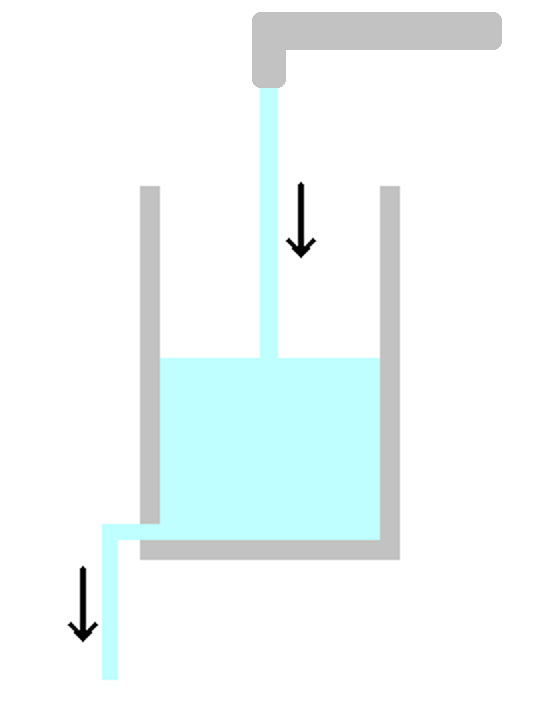
\includegraphics[height=6cm]{glass.png}
  \end{center}
  
  
\end{frame}



\begin{frame}{A leaky bucket}

  \begin{center}
    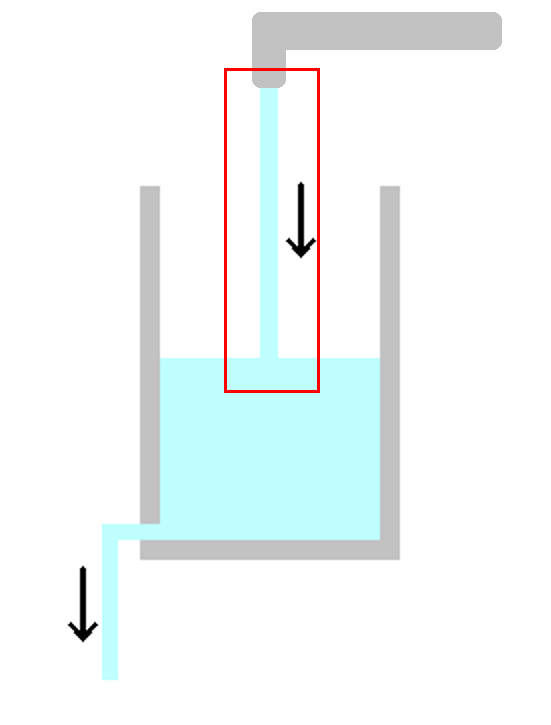
\includegraphics[height=6cm]{glass_in.png}
  \end{center}
  
  
\end{frame}

\begin{frame}{A leaky bucket}

  \begin{center}
    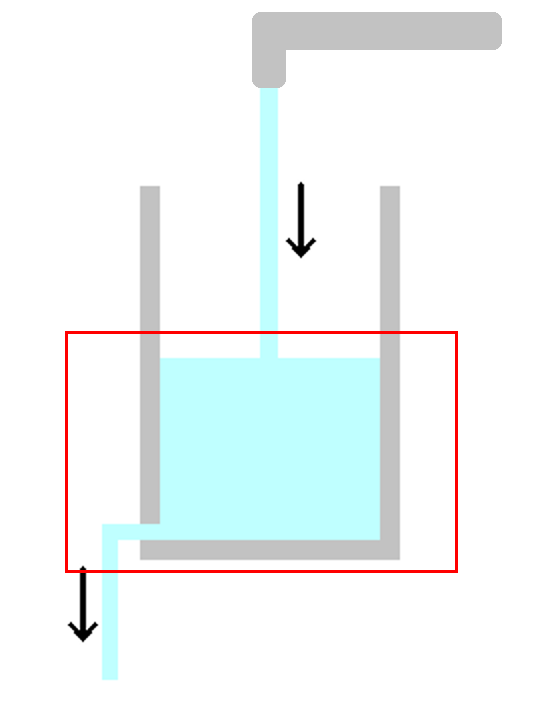
\includegraphics[height=6cm]{glass_contents.png}
  \end{center}
  
  
\end{frame}

\begin{frame}{A leaky bucket}

  \begin{center}
    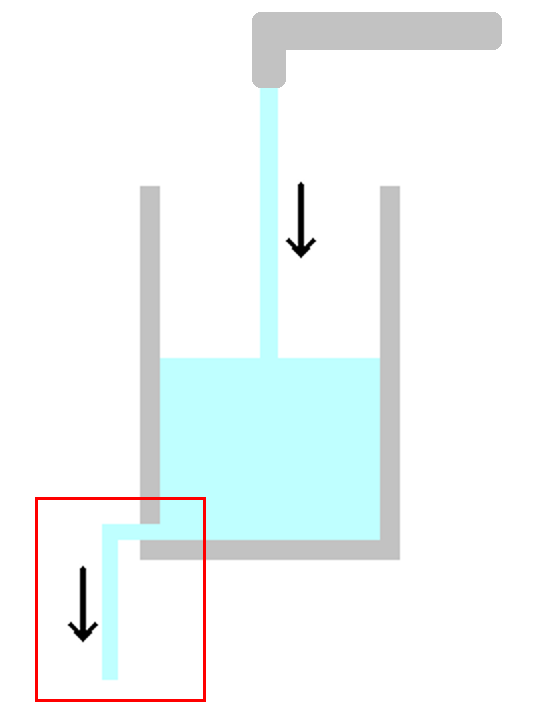
\includegraphics[height=6cm]{glass_out.png}
  \end{center}
  
  
\end{frame}


\begin{frame}{A leaky bucket - increased inflow}

  \begin{center}
    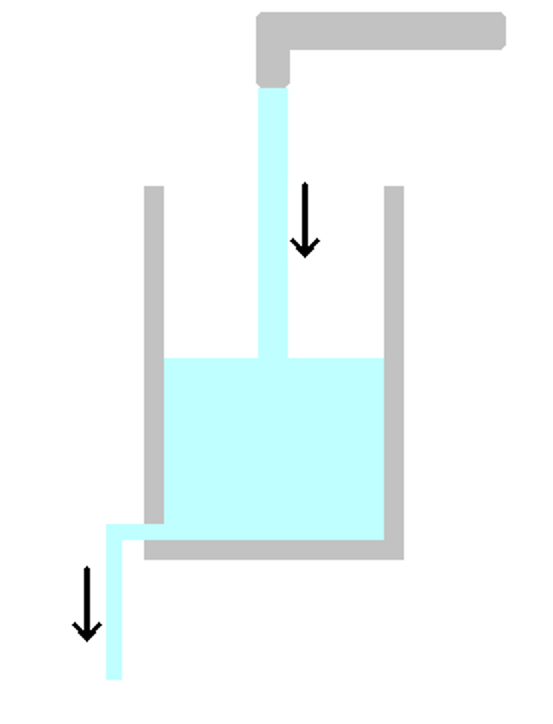
\includegraphics[height=6cm]{glass_tap_up.png}
  \end{center}
  
  
\end{frame}



\begin{frame}{A leaky bucket - increased inflow}

  \begin{center}
    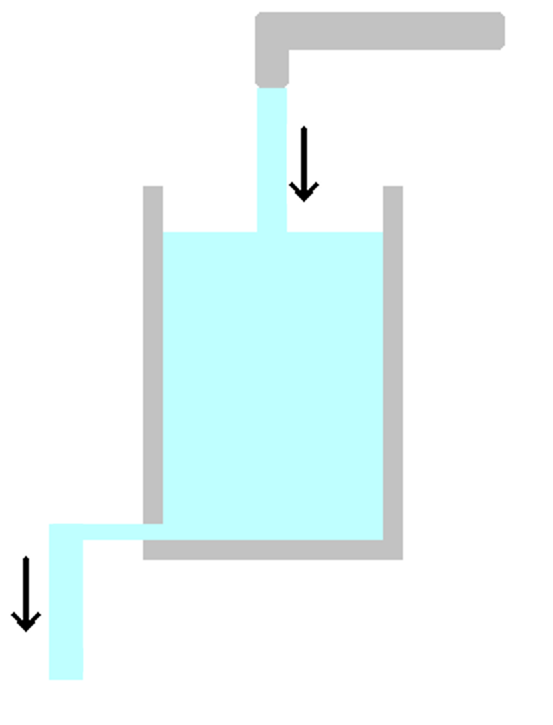
\includegraphics[height=6cm]{glass_level_up.png}
  \end{center}
  
  
\end{frame}



\begin{frame}{A leaky bucket - decreased inflow}

  \begin{center}
    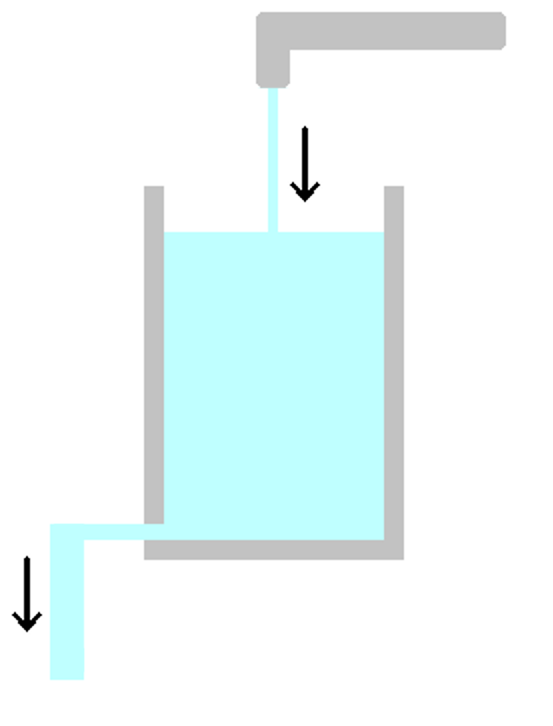
\includegraphics[height=6cm]{glass_tap_down.png}
  \end{center}
  
  
\end{frame}



\begin{frame}{A leaky bucket - decreased inflow}

  \begin{center}
    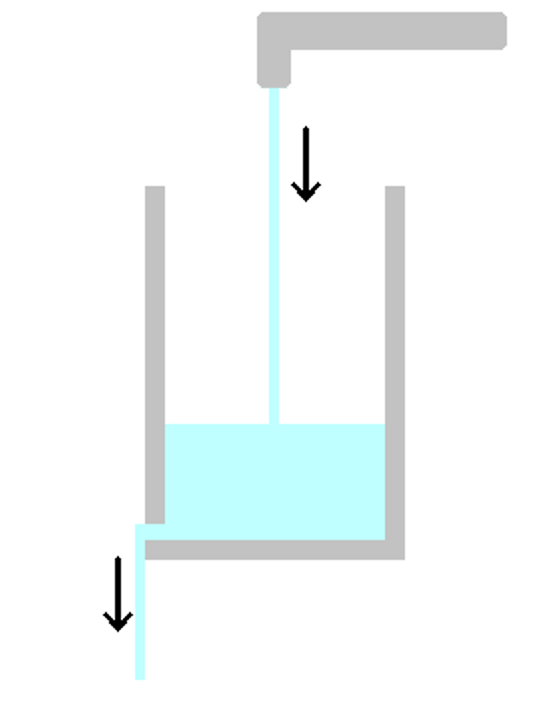
\includegraphics[height=6cm]{glass_level_down.png}
  \end{center}
  
\end{frame}


\begin{frame}{A leaky bucket - notation}
\begin{columns}
\begin{column}{0.5\textwidth}
  \begin{center}
     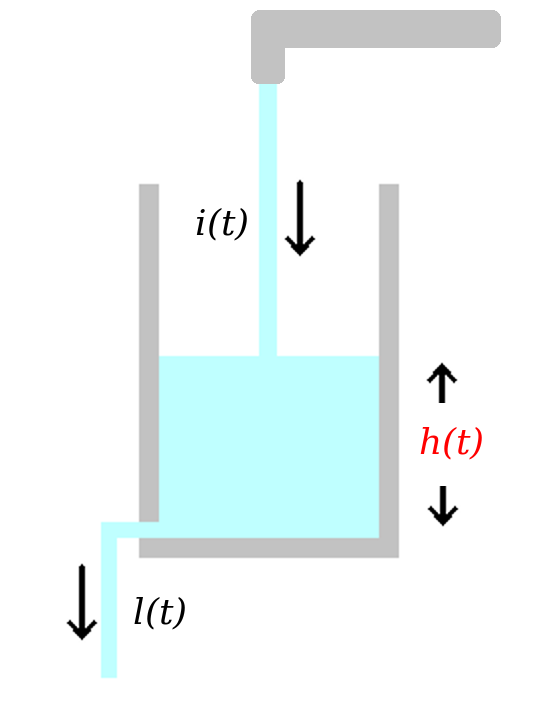
\includegraphics[height=6cm]{glass_h_red.png}      
     \end{center}
\end{column}
\begin{column}{0.5\textwidth}
\cred{} $h(t)$\color{black}{} is the height of the water.
\end{column}
\end{columns}
\end{frame}



\begin{frame}{A leaky bucket - notation}
\begin{columns}
\begin{column}{0.5\textwidth}
  \begin{center}
     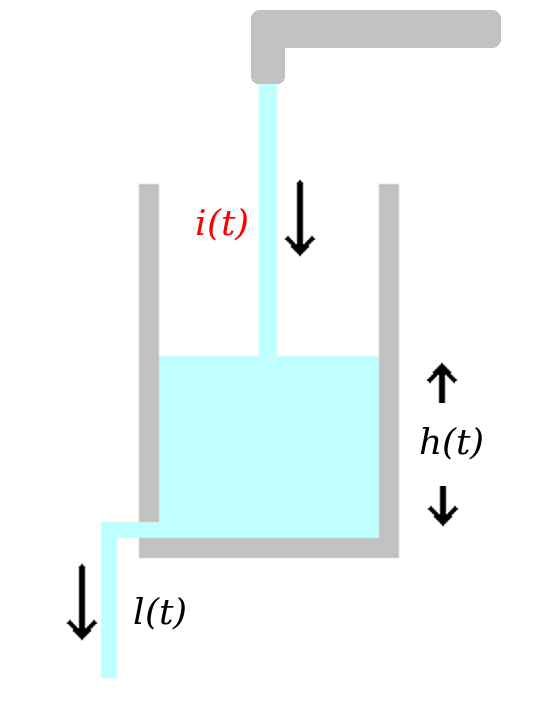
\includegraphics[height=6cm]{glass_i_red.png}      
     \end{center}
\end{column}
\begin{column}{0.5\textwidth}
  \cred{} $i(t)$\color{black}{} is the rate of flow into the
  bucket.\\[1cm] It is a \textsl{rate} so it would be meaured in
  volume per time, for example, \crish$Ls^{-1}$\cbla.
\end{column}
\end{columns}
\end{frame}


\begin{frame}{A leaky bucket - notation}
\begin{columns}
\begin{column}{0.5\textwidth}
  \begin{center}
     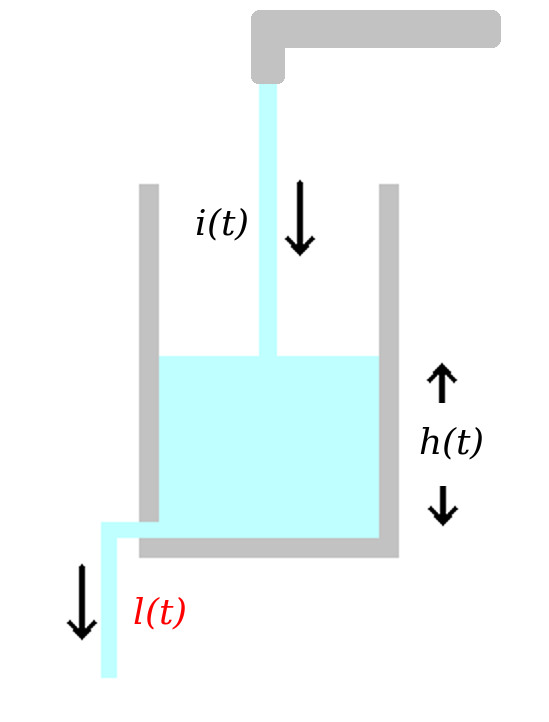
\includegraphics[height=6cm]{glass_l_red.png}      
     \end{center}
\end{column}
\begin{column}{0.5\textwidth}
  \cred{} $l(t)$\color{black}{} is the rate of flow out of the
  bucket.\\[1cm] It is a \textsl{rate} so it would be meaured in
  volume per time, for example, \crish$Ls^{-1}$\cbla.
  
\end{column}
\end{columns}
\end{frame}


\begin{frame}{A leaky bucket - leak}
\begin{columns}
\begin{column}{0.5\textwidth}
  \begin{center}
     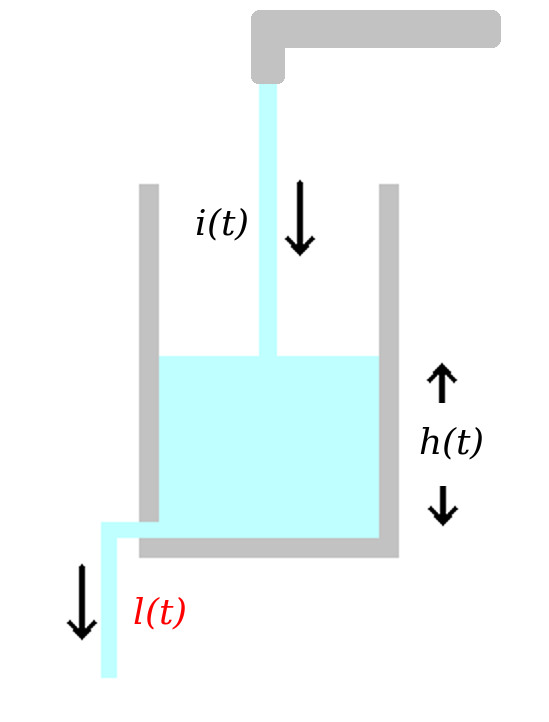
\includegraphics[height=6cm]{glass_l_red.png}      
     \end{center}
\end{column}
\begin{column}{0.5\textwidth}
  The speed of the leak depends on the hieght of the water so\crish
  $$l(t)\propto h(t)$$
  \cbla{}or, adding a constant of proportionality\crish
  $$l(t)=Gh(t)$$
  \cbla{}where \crish{}$G$\cbla{} depends on some physics stuff we aren't interested in here.


  
\end{column}
\end{columns}
\end{frame}


\begin{frame}{A leaky bucket - net flow}
\begin{columns}
\begin{column}{0.5\textwidth}
  \begin{center}
     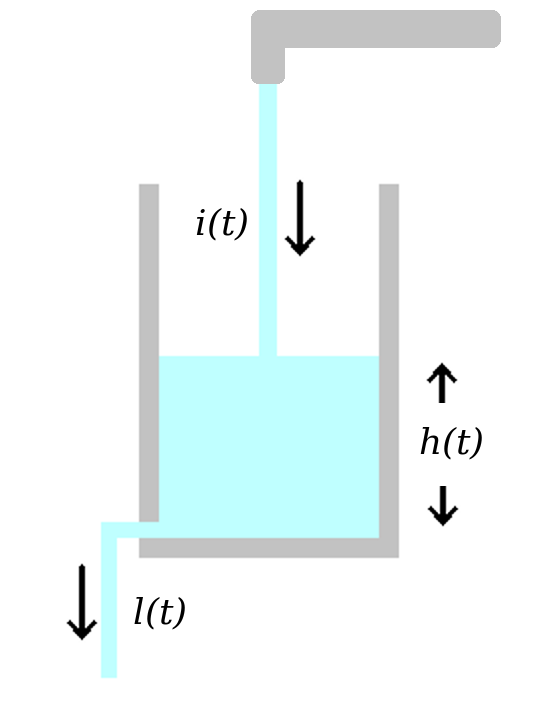
\includegraphics[height=6cm]{glass_notation.png}      
     \end{center}
\end{column}
\begin{column}{0.5\textwidth}
  The net flow into the bucket is therefore\crish
  $$i(t)- l(t)$$
  \cbla{}or,\crish{} 
  $$i(t)-Gh(t)$$
  \cbla{}and, remember this is a flow, so it is measured in volume per time.

\end{column}
\end{columns}
\end{frame}


\begin{frame}{A leaky bucket - volumn}
\begin{columns}
\begin{column}{0.5\textwidth}
  \begin{center}
     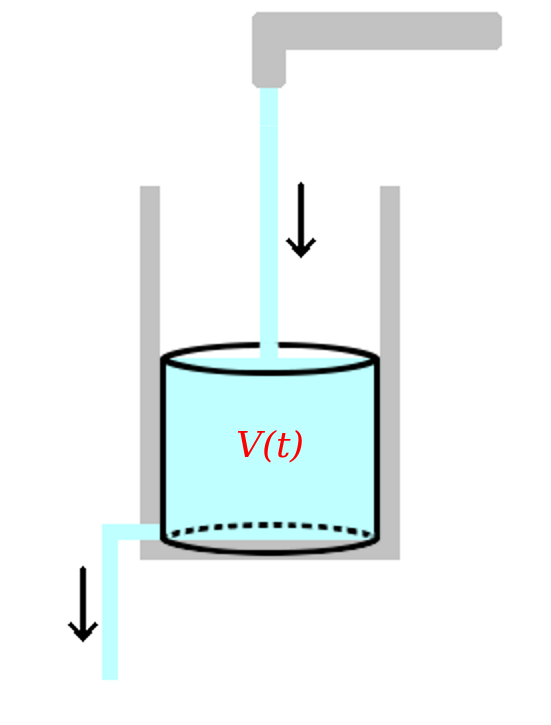
\includegraphics[height=6cm]{glass_volume_notation.png}      
     \end{center}
\end{column}
\begin{column}{0.5\textwidth}
  The net flow changes the volume of water.\\[0.5cm]
  
The volume depends on the height:
  \crish
  $$V(t)=Ch(t)$$ \cbla{}where \crish$C$\cbla{} is a constant.\\[0.5cm]
  In the case of a
  cylindrical bucket, using the formula for the volumn of a cylinder
  tells us that \crish$C=\pi r^2$\cbla{} where \crish$r$\cbla{} is the
  radius of the bucket; but we'll just call it \crish$C$\cbla.
\end{column}
\end{columns}
\end{frame}

\begin{frame}{Equation for a leaky bucket}

  The rate of change of the volume is equal to the net inflow. The
  rate of change is given by the derivative:\crish
  $$\frac{dV}{dt}=i-Gh$$
  \cbla{}
\end{frame}


\begin{frame}{Equation for a leaky bucket}

  The rate of change of the volume is equal to the net inflow. The
  rate of change is given by the derivative:\crish
  $$\frac{dV}{dt}=i-Gh$$
  \cbla{}Notice that when we want to emphasis that something changes with time we write the brackets \crish$t$\cbla, like \crish$h(t)$\cbla{} but at other times we leave it out to stop making equations look to cluttered!\cbla.
\end{frame}


\begin{frame}{Equation for a leaky bucket}
  \crish
  $$\frac{dV}{dt}=i-Gh$$
  \cbla{}Substituting \crish$V=Ch$\cbla{} we get\crish
  $$\frac{d\cblu Ch\crish}{dt}=i-Gh$$
  \cbla{}Since \crish$C$\cbla{} is a constant this means\crish
  $$C\frac{dh}{dt}=i-Gh$$\cbla
  This is our basic equation for the height of the water in a leaky bucket.
\end{frame}


\begin{frame}{Equation for a leaky bucket}
  Let's rewrite this equation as 
  \crish
  $$\cblu\tau\crish\frac{dh}{dt}=\frac{1}{G}i-h$$\cbla where
  \cblu$\tau\crish{}=C/G$\cbla{}.\\[1cm]
  This notation is used because
  \cblu$\tau$\cbla{} is a timescale and \crish$\tau$\cbla{} is the
  Greek equivalent of \crish$t$\cbla. If you work out all the units for the constants \crish$C$\cbla{} and \crish$G$\cbla{} you can see \cblu$\tau$\cbla{} has units of time; it also balances the \textsl{per time} in the derivative. 
\end{frame}

\begin{frame}{Constant input}
  First lets looks at what happens when the water is flowing in at a constant rate, that is when \crish$i$\cbla{} doesn't change with time; lets write\cblu{}
  $$i=\bar{\i}$$\cbla{} when the input is constant.
\end{frame}

\begin{frame}{Behaviour of the equation}
  \crish
  $$\tau\frac{dh}{dt}=\frac{1}{G}\bar{\i}-h$$\cbla If
  \cblu{}$\bar{\i}=Gh$\cbla{} then \cblu{}$dh/dt=0$\cbla{}. This is
  the equilibrium where the inflow is equal to the outflow.
\end{frame}

\begin{frame}{Behaviour of the equation}
  \crish
  $$\tau\frac{dh}{dt}=\frac{1}{G}\bar{\i}-h$$\cbla If
  \cblu{}$\bar{\i}<Gh$\cbla{} then \cblu{}$dh/dt<0$\cbla{} and the
  level of the water falls; so if the water height is too high it
  decreases towards equilibrium.
\end{frame}


\begin{frame}{A leaky bucket - decreased inflow}

  \begin{center}
    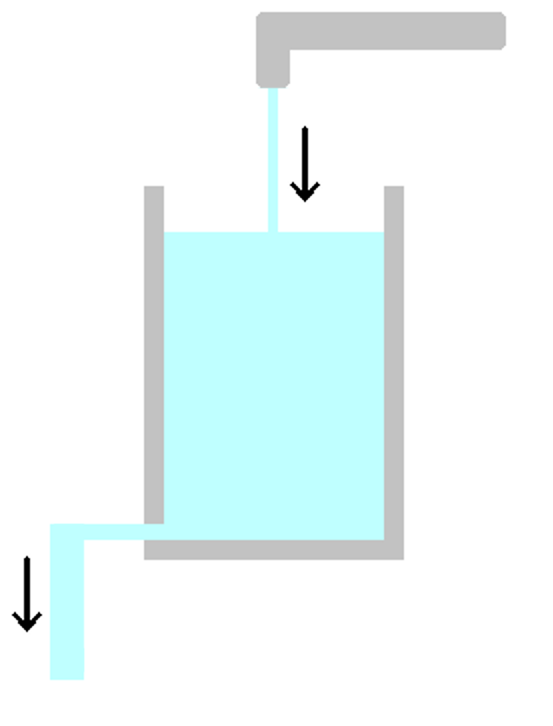
\includegraphics[height=6cm]{glass_tap_down.png}
  \end{center}
  
  
\end{frame}



\begin{frame}{A leaky bucket - decreased inflow}

  \begin{center}
    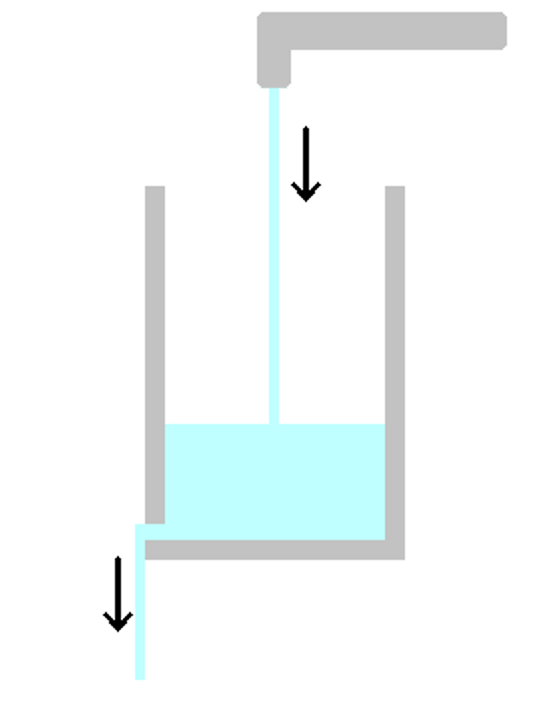
\includegraphics[height=6cm]{glass_level_down.png}
  \end{center}
  
\end{frame}


\begin{frame}{Behaviour of the equation}
  \crish
  $$\tau\frac{dh}{dt}=\frac{1}{G}\bar{\i}-h$$\cbla Conversely if
  \cblu{}$\bar{\i}>Gh$\cbla{} then \cblu{}$dh/dt>0$\cbla{} and the
  level of the water falls; so if the water height is too low it
  increases towards equilibrium.
\end{frame}


\begin{frame}{Behaviour of the equation}
  \crish
  $$\tau\frac{dh}{dt}=\frac{1}{G}\bar{\i}-h$$\cbla Notice also that the more
  \crish{}$\bar{\i}>Gh$\cbla{} the more \crish{}$dh/dt>0$\cbla{} and \textsl{visa versa} for \crish{}$\bar{\i}<Gh$\cbla: the further the hieght is from the equilibrium, the faster it goes towards equilibrium.
\end{frame}


\begin{frame}{Solution of the equation}
  In fact we can solve the equation:\crish{}
$$h(t)=[h(0)-\bar{\i}/G]e^{-t/\tau}+\bar{\i}/G$$
\cbla{}Solving the equation isn't hard but we won't look at it here.
\end{frame}


\begin{frame}{Solution of the equation}
  \crish{}
$$h(t)=[\cblu{}h(0)\crish{}-\bar{\i}/G]e^{-t/\tau}+\bar{\i}/G$$
\cbla{}where \cblu$h(0)$\cbla{} is the initial value of \crish$h$\cbla{}; that is the value it starts at.
\end{frame}


\begin{frame}{Solution of the equation}
  \crish{}
$$h(t)=[h(0)-\bar{\i}/G]\cblu{}e^{-t/\tau}\crish{}+\bar{\i}/G$$
\cbla{}Here\cblu
$$e^{-t/\tau}$$
\cbla{}is the \cblu{}exponential function\cbla{}; sometimes it is written in another form:
\cblu
$$\exp{\left(-\frac{t}{\tau}\right)}$$
\cbla{}and is one of the start function like sine and cosine.
\end{frame}

\begin{frame}{Exponential}
  \crish$$y=e^{-t}$$
  \begin{center}
    % GNUPLOT: LaTeX picture with Postscript
\begingroup
  \makeatletter
  \providecommand\color[2][]{%
    \GenericError{(gnuplot) \space\space\space\@spaces}{%
      Package color not loaded in conjunction with
      terminal option `colourtext'%
    }{See the gnuplot documentation for explanation.%
    }{Either use 'blacktext' in gnuplot or load the package
      color.sty in LaTeX.}%
    \renewcommand\color[2][]{}%
  }%
  \providecommand\includegraphics[2][]{%
    \GenericError{(gnuplot) \space\space\space\@spaces}{%
      Package graphicx or graphics not loaded%
    }{See the gnuplot documentation for explanation.%
    }{The gnuplot epslatex terminal needs graphicx.sty or graphics.sty.}%
    \renewcommand\includegraphics[2][]{}%
  }%
  \providecommand\rotatebox[2]{#2}%
  \@ifundefined{ifGPcolor}{%
    \newif\ifGPcolor
    \GPcolorfalse
  }{}%
  \@ifundefined{ifGPblacktext}{%
    \newif\ifGPblacktext
    \GPblacktexttrue
  }{}%
  % define a \g@addto@macro without @ in the name:
  \let\gplgaddtomacro\g@addto@macro
  % define empty templates for all commands taking text:
  \gdef\gplbacktext{}%
  \gdef\gplfronttext{}%
  \makeatother
  \ifGPblacktext
    % no textcolor at all
    \def\colorrgb#1{}%
    \def\colorgray#1{}%
  \else
    % gray or color?
    \ifGPcolor
      \def\colorrgb#1{\color[rgb]{#1}}%
      \def\colorgray#1{\color[gray]{#1}}%
      \expandafter\def\csname LTw\endcsname{\color{white}}%
      \expandafter\def\csname LTb\endcsname{\color{black}}%
      \expandafter\def\csname LTa\endcsname{\color{black}}%
      \expandafter\def\csname LT0\endcsname{\color[rgb]{1,0,0}}%
      \expandafter\def\csname LT1\endcsname{\color[rgb]{0,1,0}}%
      \expandafter\def\csname LT2\endcsname{\color[rgb]{0,0,1}}%
      \expandafter\def\csname LT3\endcsname{\color[rgb]{1,0,1}}%
      \expandafter\def\csname LT4\endcsname{\color[rgb]{0,1,1}}%
      \expandafter\def\csname LT5\endcsname{\color[rgb]{1,1,0}}%
      \expandafter\def\csname LT6\endcsname{\color[rgb]{0,0,0}}%
      \expandafter\def\csname LT7\endcsname{\color[rgb]{1,0.3,0}}%
      \expandafter\def\csname LT8\endcsname{\color[rgb]{0.5,0.5,0.5}}%
    \else
      % gray
      \def\colorrgb#1{\color{black}}%
      \def\colorgray#1{\color[gray]{#1}}%
      \expandafter\def\csname LTw\endcsname{\color{white}}%
      \expandafter\def\csname LTb\endcsname{\color{black}}%
      \expandafter\def\csname LTa\endcsname{\color{black}}%
      \expandafter\def\csname LT0\endcsname{\color{black}}%
      \expandafter\def\csname LT1\endcsname{\color{black}}%
      \expandafter\def\csname LT2\endcsname{\color{black}}%
      \expandafter\def\csname LT3\endcsname{\color{black}}%
      \expandafter\def\csname LT4\endcsname{\color{black}}%
      \expandafter\def\csname LT5\endcsname{\color{black}}%
      \expandafter\def\csname LT6\endcsname{\color{black}}%
      \expandafter\def\csname LT7\endcsname{\color{black}}%
      \expandafter\def\csname LT8\endcsname{\color{black}}%
    \fi
  \fi
  \setlength{\unitlength}{0.0500bp}%
  \begin{picture}(4320.00,3024.00)%
    \gplgaddtomacro\gplbacktext{%
      \csname LTb\endcsname%
      \put(1078,704){\makebox(0,0)[r]{\strut{} 0}}%
      \put(1078,1218){\makebox(0,0)[r]{\strut{} 0.25}}%
      \put(1078,1732){\makebox(0,0)[r]{\strut{} 0.5}}%
      \put(1078,2245){\makebox(0,0)[r]{\strut{} 0.75}}%
      \put(1078,2759){\makebox(0,0)[r]{\strut{} 1}}%
      \put(1210,484){\makebox(0,0){\strut{} 0}}%
      \put(1753,484){\makebox(0,0){\strut{} 1}}%
      \put(2295,484){\makebox(0,0){\strut{} 2}}%
      \put(2838,484){\makebox(0,0){\strut{} 3}}%
      \put(3380,484){\makebox(0,0){\strut{} 4}}%
      \put(3923,484){\makebox(0,0){\strut{} 5}}%
      \put(176,1731){\rotatebox{-270}{\makebox(0,0){\strut{}$y$}}}%
      \put(2566,154){\makebox(0,0){\strut{}$t$}}%
    }%
    \gplgaddtomacro\gplfronttext{%
    }%
    \gplbacktext
    \put(0,0){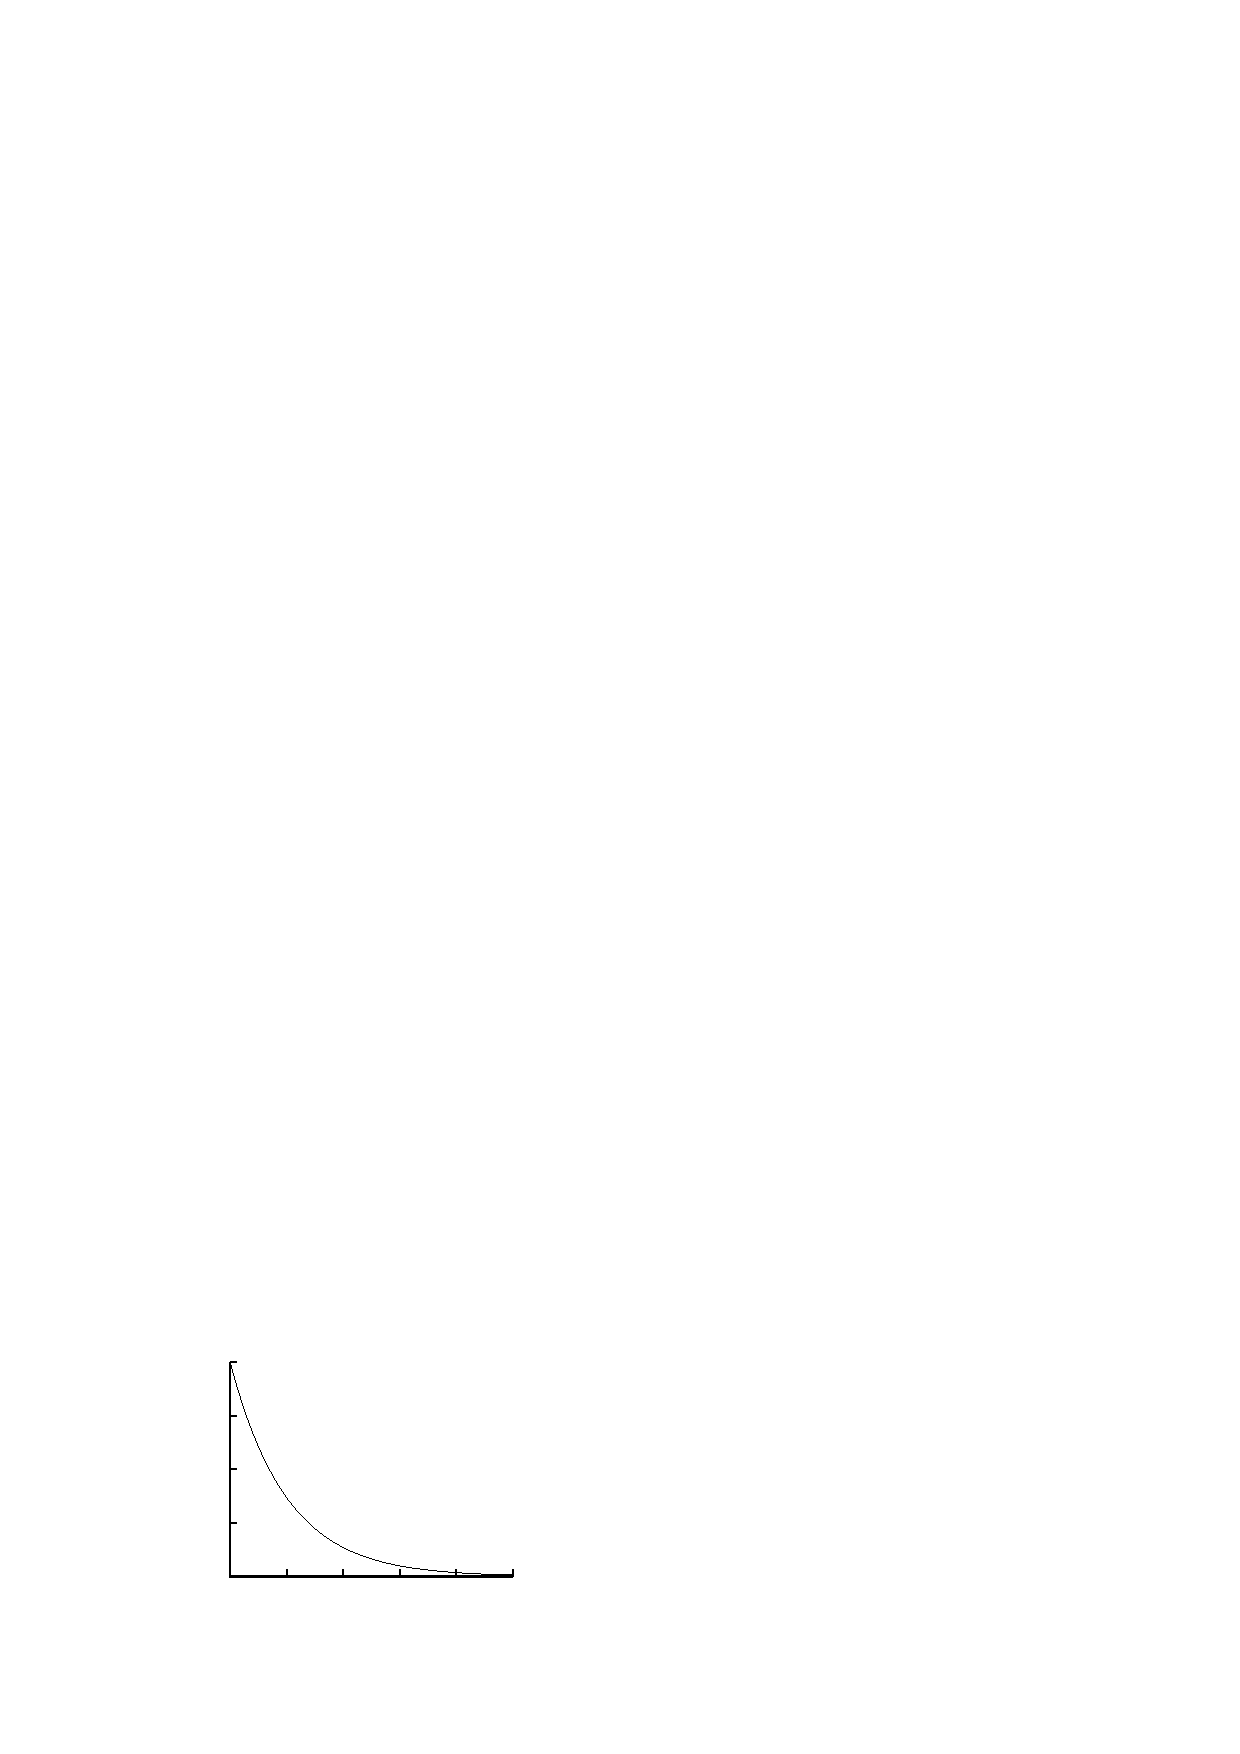
\includegraphics{exp}}%
    \gplfronttext
  \end{picture}%
\endgroup

  \end{center}
  \end{frame}


\begin{frame}{Exponential}
  \crish$$y=e^{-t/2}$$
  \begin{center}
    % GNUPLOT: LaTeX picture with Postscript
\begingroup
  \makeatletter
  \providecommand\color[2][]{%
    \GenericError{(gnuplot) \space\space\space\@spaces}{%
      Package color not loaded in conjunction with
      terminal option `colourtext'%
    }{See the gnuplot documentation for explanation.%
    }{Either use 'blacktext' in gnuplot or load the package
      color.sty in LaTeX.}%
    \renewcommand\color[2][]{}%
  }%
  \providecommand\includegraphics[2][]{%
    \GenericError{(gnuplot) \space\space\space\@spaces}{%
      Package graphicx or graphics not loaded%
    }{See the gnuplot documentation for explanation.%
    }{The gnuplot epslatex terminal needs graphicx.sty or graphics.sty.}%
    \renewcommand\includegraphics[2][]{}%
  }%
  \providecommand\rotatebox[2]{#2}%
  \@ifundefined{ifGPcolor}{%
    \newif\ifGPcolor
    \GPcolorfalse
  }{}%
  \@ifundefined{ifGPblacktext}{%
    \newif\ifGPblacktext
    \GPblacktexttrue
  }{}%
  % define a \g@addto@macro without @ in the name:
  \let\gplgaddtomacro\g@addto@macro
  % define empty templates for all commands taking text:
  \gdef\gplbacktext{}%
  \gdef\gplfronttext{}%
  \makeatother
  \ifGPblacktext
    % no textcolor at all
    \def\colorrgb#1{}%
    \def\colorgray#1{}%
  \else
    % gray or color?
    \ifGPcolor
      \def\colorrgb#1{\color[rgb]{#1}}%
      \def\colorgray#1{\color[gray]{#1}}%
      \expandafter\def\csname LTw\endcsname{\color{white}}%
      \expandafter\def\csname LTb\endcsname{\color{black}}%
      \expandafter\def\csname LTa\endcsname{\color{black}}%
      \expandafter\def\csname LT0\endcsname{\color[rgb]{1,0,0}}%
      \expandafter\def\csname LT1\endcsname{\color[rgb]{0,1,0}}%
      \expandafter\def\csname LT2\endcsname{\color[rgb]{0,0,1}}%
      \expandafter\def\csname LT3\endcsname{\color[rgb]{1,0,1}}%
      \expandafter\def\csname LT4\endcsname{\color[rgb]{0,1,1}}%
      \expandafter\def\csname LT5\endcsname{\color[rgb]{1,1,0}}%
      \expandafter\def\csname LT6\endcsname{\color[rgb]{0,0,0}}%
      \expandafter\def\csname LT7\endcsname{\color[rgb]{1,0.3,0}}%
      \expandafter\def\csname LT8\endcsname{\color[rgb]{0.5,0.5,0.5}}%
    \else
      % gray
      \def\colorrgb#1{\color{black}}%
      \def\colorgray#1{\color[gray]{#1}}%
      \expandafter\def\csname LTw\endcsname{\color{white}}%
      \expandafter\def\csname LTb\endcsname{\color{black}}%
      \expandafter\def\csname LTa\endcsname{\color{black}}%
      \expandafter\def\csname LT0\endcsname{\color{black}}%
      \expandafter\def\csname LT1\endcsname{\color{black}}%
      \expandafter\def\csname LT2\endcsname{\color{black}}%
      \expandafter\def\csname LT3\endcsname{\color{black}}%
      \expandafter\def\csname LT4\endcsname{\color{black}}%
      \expandafter\def\csname LT5\endcsname{\color{black}}%
      \expandafter\def\csname LT6\endcsname{\color{black}}%
      \expandafter\def\csname LT7\endcsname{\color{black}}%
      \expandafter\def\csname LT8\endcsname{\color{black}}%
    \fi
  \fi
  \setlength{\unitlength}{0.0500bp}%
  \begin{picture}(4320.00,3024.00)%
    \gplgaddtomacro\gplbacktext{%
      \csname LTb\endcsname%
      \put(1078,704){\makebox(0,0)[r]{\strut{} 0}}%
      \put(1078,1218){\makebox(0,0)[r]{\strut{} 0.25}}%
      \put(1078,1732){\makebox(0,0)[r]{\strut{} 0.5}}%
      \put(1078,2245){\makebox(0,0)[r]{\strut{} 0.75}}%
      \put(1078,2759){\makebox(0,0)[r]{\strut{} 1}}%
      \put(1210,484){\makebox(0,0){\strut{} 0}}%
      \put(1753,484){\makebox(0,0){\strut{} 1}}%
      \put(2295,484){\makebox(0,0){\strut{} 2}}%
      \put(2838,484){\makebox(0,0){\strut{} 3}}%
      \put(3380,484){\makebox(0,0){\strut{} 4}}%
      \put(3923,484){\makebox(0,0){\strut{} 5}}%
      \put(176,1731){\rotatebox{-270}{\makebox(0,0){\strut{}$y$}}}%
      \put(2566,154){\makebox(0,0){\strut{}$t$}}%
    }%
    \gplgaddtomacro\gplfronttext{%
    }%
    \gplbacktext
    \put(0,0){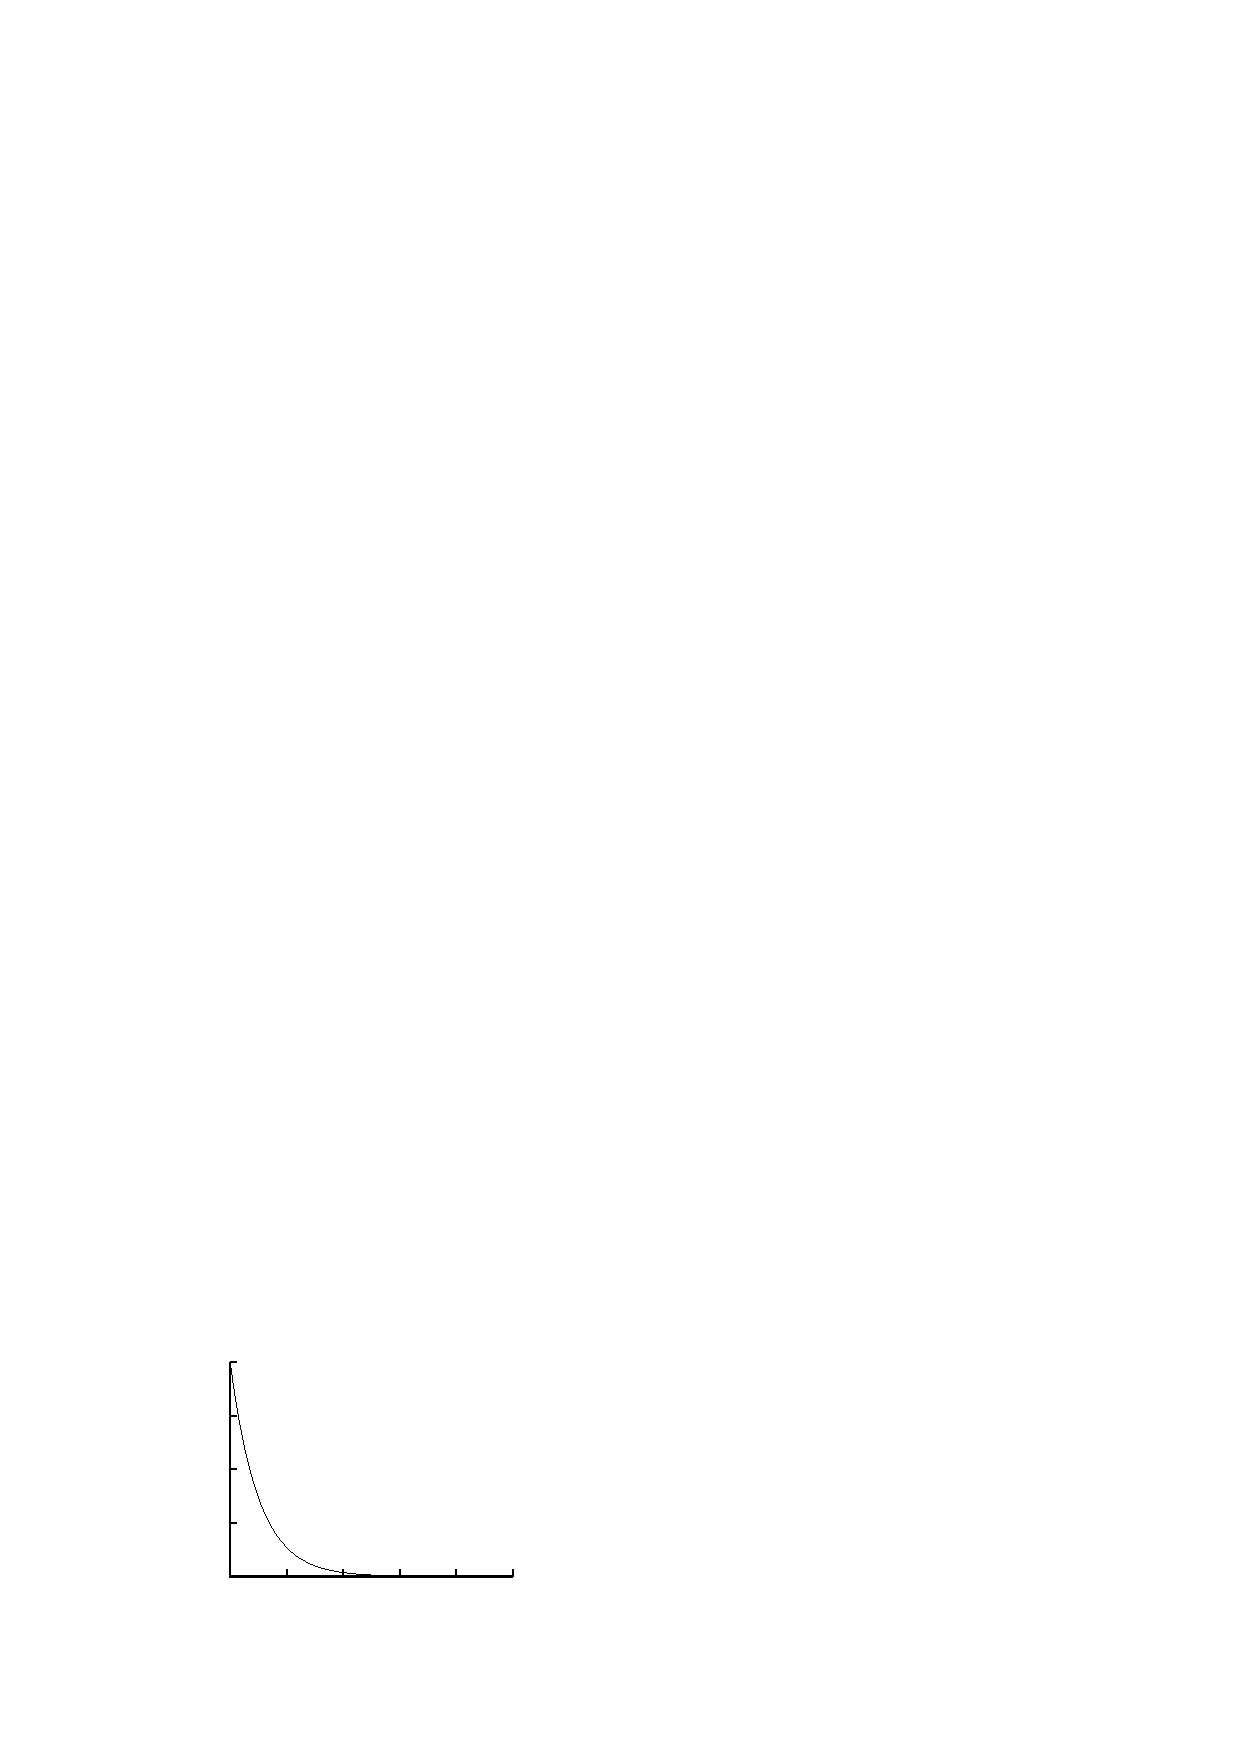
\includegraphics{exptau2}}%
    \gplfronttext
  \end{picture}%
\endgroup

  \end{center}
  \end{frame}


\begin{frame}{Exponential}
  \crish$$y=e^{-2t}$$
  \begin{center}
    % GNUPLOT: LaTeX picture with Postscript
\begingroup
  \makeatletter
  \providecommand\color[2][]{%
    \GenericError{(gnuplot) \space\space\space\@spaces}{%
      Package color not loaded in conjunction with
      terminal option `colourtext'%
    }{See the gnuplot documentation for explanation.%
    }{Either use 'blacktext' in gnuplot or load the package
      color.sty in LaTeX.}%
    \renewcommand\color[2][]{}%
  }%
  \providecommand\includegraphics[2][]{%
    \GenericError{(gnuplot) \space\space\space\@spaces}{%
      Package graphicx or graphics not loaded%
    }{See the gnuplot documentation for explanation.%
    }{The gnuplot epslatex terminal needs graphicx.sty or graphics.sty.}%
    \renewcommand\includegraphics[2][]{}%
  }%
  \providecommand\rotatebox[2]{#2}%
  \@ifundefined{ifGPcolor}{%
    \newif\ifGPcolor
    \GPcolorfalse
  }{}%
  \@ifundefined{ifGPblacktext}{%
    \newif\ifGPblacktext
    \GPblacktexttrue
  }{}%
  % define a \g@addto@macro without @ in the name:
  \let\gplgaddtomacro\g@addto@macro
  % define empty templates for all commands taking text:
  \gdef\gplbacktext{}%
  \gdef\gplfronttext{}%
  \makeatother
  \ifGPblacktext
    % no textcolor at all
    \def\colorrgb#1{}%
    \def\colorgray#1{}%
  \else
    % gray or color?
    \ifGPcolor
      \def\colorrgb#1{\color[rgb]{#1}}%
      \def\colorgray#1{\color[gray]{#1}}%
      \expandafter\def\csname LTw\endcsname{\color{white}}%
      \expandafter\def\csname LTb\endcsname{\color{black}}%
      \expandafter\def\csname LTa\endcsname{\color{black}}%
      \expandafter\def\csname LT0\endcsname{\color[rgb]{1,0,0}}%
      \expandafter\def\csname LT1\endcsname{\color[rgb]{0,1,0}}%
      \expandafter\def\csname LT2\endcsname{\color[rgb]{0,0,1}}%
      \expandafter\def\csname LT3\endcsname{\color[rgb]{1,0,1}}%
      \expandafter\def\csname LT4\endcsname{\color[rgb]{0,1,1}}%
      \expandafter\def\csname LT5\endcsname{\color[rgb]{1,1,0}}%
      \expandafter\def\csname LT6\endcsname{\color[rgb]{0,0,0}}%
      \expandafter\def\csname LT7\endcsname{\color[rgb]{1,0.3,0}}%
      \expandafter\def\csname LT8\endcsname{\color[rgb]{0.5,0.5,0.5}}%
    \else
      % gray
      \def\colorrgb#1{\color{black}}%
      \def\colorgray#1{\color[gray]{#1}}%
      \expandafter\def\csname LTw\endcsname{\color{white}}%
      \expandafter\def\csname LTb\endcsname{\color{black}}%
      \expandafter\def\csname LTa\endcsname{\color{black}}%
      \expandafter\def\csname LT0\endcsname{\color{black}}%
      \expandafter\def\csname LT1\endcsname{\color{black}}%
      \expandafter\def\csname LT2\endcsname{\color{black}}%
      \expandafter\def\csname LT3\endcsname{\color{black}}%
      \expandafter\def\csname LT4\endcsname{\color{black}}%
      \expandafter\def\csname LT5\endcsname{\color{black}}%
      \expandafter\def\csname LT6\endcsname{\color{black}}%
      \expandafter\def\csname LT7\endcsname{\color{black}}%
      \expandafter\def\csname LT8\endcsname{\color{black}}%
    \fi
  \fi
  \setlength{\unitlength}{0.0500bp}%
  \begin{picture}(4320.00,3024.00)%
    \gplgaddtomacro\gplbacktext{%
      \csname LTb\endcsname%
      \put(1078,704){\makebox(0,0)[r]{\strut{} 0}}%
      \put(1078,1218){\makebox(0,0)[r]{\strut{} 0.25}}%
      \put(1078,1732){\makebox(0,0)[r]{\strut{} 0.5}}%
      \put(1078,2245){\makebox(0,0)[r]{\strut{} 0.75}}%
      \put(1078,2759){\makebox(0,0)[r]{\strut{} 1}}%
      \put(1210,484){\makebox(0,0){\strut{} 0}}%
      \put(1753,484){\makebox(0,0){\strut{} 1}}%
      \put(2295,484){\makebox(0,0){\strut{} 2}}%
      \put(2838,484){\makebox(0,0){\strut{} 3}}%
      \put(3380,484){\makebox(0,0){\strut{} 4}}%
      \put(3923,484){\makebox(0,0){\strut{} 5}}%
      \put(176,1731){\rotatebox{-270}{\makebox(0,0){\strut{}$y$}}}%
      \put(2566,154){\makebox(0,0){\strut{}$t$}}%
    }%
    \gplgaddtomacro\gplfronttext{%
    }%
    \gplbacktext
    \put(0,0){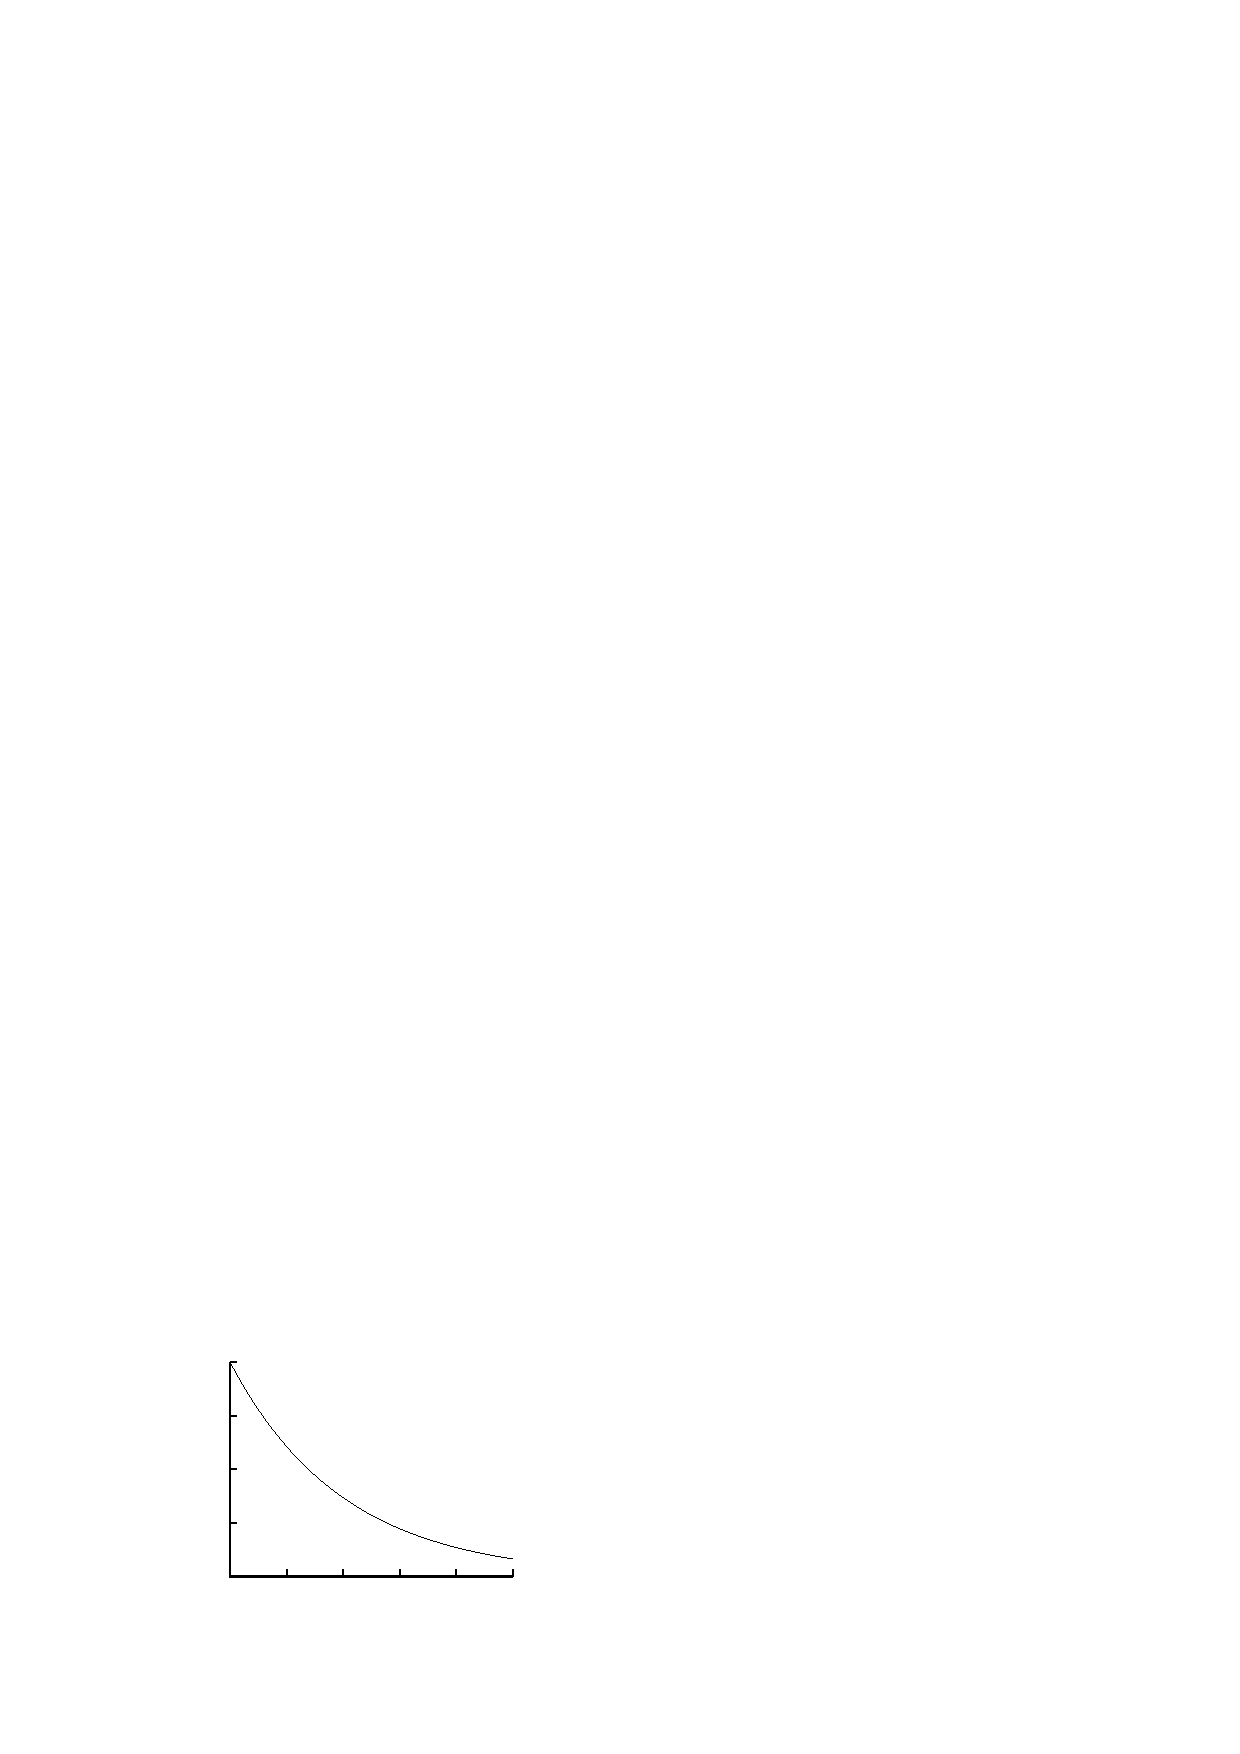
\includegraphics{exptauhalf}}%
    \gplfronttext
  \end{picture}%
\endgroup

  \end{center}
  \end{frame}



\begin{frame}{Solution of the equation}
  \crish{}
$$h(t)=[h(0)-\bar{\i}/G]\cblu{}e^{-t/\tau}\crish{}+\bar{\i}/G$$
\cbla{}Here\cblu
$$e^{-t/\tau}$$
\cbla{}so the exponential decays away.
\end{frame}


\begin{frame}{Solution of the equation}
  \crish{}
$$h(t)=[h(0)-\bar{\i}/G]e^{-t/\tau}+\cblu{}\bar{\i}/G\crish{}$$
\cbla{}Here\cblu
$$e^{-t/\tau}$$
\cbla{}so the exponential decays away and the height approaches its equilibrium value of \cblu$\bar{\i}/G$\crish.
\end{frame}

\begin{frame}{Exponential relaxation}
  These dynamics are very common and are sometimes called \textsl{exponential relaxation to the equilibrium}. Here are some examples with \crish$\bar{\i}=G$\cbla, \crish$\tau=1$\cbla{} and three different initial values \crish$h(0)$\cbla.
\begin{center}
% GNUPLOT: LaTeX picture with Postscript
\begingroup
  \makeatletter
  \providecommand\color[2][]{%
    \GenericError{(gnuplot) \space\space\space\@spaces}{%
      Package color not loaded in conjunction with
      terminal option `colourtext'%
    }{See the gnuplot documentation for explanation.%
    }{Either use 'blacktext' in gnuplot or load the package
      color.sty in LaTeX.}%
    \renewcommand\color[2][]{}%
  }%
  \providecommand\includegraphics[2][]{%
    \GenericError{(gnuplot) \space\space\space\@spaces}{%
      Package graphicx or graphics not loaded%
    }{See the gnuplot documentation for explanation.%
    }{The gnuplot epslatex terminal needs graphicx.sty or graphics.sty.}%
    \renewcommand\includegraphics[2][]{}%
  }%
  \providecommand\rotatebox[2]{#2}%
  \@ifundefined{ifGPcolor}{%
    \newif\ifGPcolor
    \GPcolorfalse
  }{}%
  \@ifundefined{ifGPblacktext}{%
    \newif\ifGPblacktext
    \GPblacktexttrue
  }{}%
  % define a \g@addto@macro without @ in the name:
  \let\gplgaddtomacro\g@addto@macro
  % define empty templates for all commands taking text:
  \gdef\gplbacktext{}%
  \gdef\gplfronttext{}%
  \makeatother
  \ifGPblacktext
    % no textcolor at all
    \def\colorrgb#1{}%
    \def\colorgray#1{}%
  \else
    % gray or color?
    \ifGPcolor
      \def\colorrgb#1{\color[rgb]{#1}}%
      \def\colorgray#1{\color[gray]{#1}}%
      \expandafter\def\csname LTw\endcsname{\color{white}}%
      \expandafter\def\csname LTb\endcsname{\color{black}}%
      \expandafter\def\csname LTa\endcsname{\color{black}}%
      \expandafter\def\csname LT0\endcsname{\color[rgb]{1,0,0}}%
      \expandafter\def\csname LT1\endcsname{\color[rgb]{0,1,0}}%
      \expandafter\def\csname LT2\endcsname{\color[rgb]{0,0,1}}%
      \expandafter\def\csname LT3\endcsname{\color[rgb]{1,0,1}}%
      \expandafter\def\csname LT4\endcsname{\color[rgb]{0,1,1}}%
      \expandafter\def\csname LT5\endcsname{\color[rgb]{1,1,0}}%
      \expandafter\def\csname LT6\endcsname{\color[rgb]{0,0,0}}%
      \expandafter\def\csname LT7\endcsname{\color[rgb]{1,0.3,0}}%
      \expandafter\def\csname LT8\endcsname{\color[rgb]{0.5,0.5,0.5}}%
    \else
      % gray
      \def\colorrgb#1{\color{black}}%
      \def\colorgray#1{\color[gray]{#1}}%
      \expandafter\def\csname LTw\endcsname{\color{white}}%
      \expandafter\def\csname LTb\endcsname{\color{black}}%
      \expandafter\def\csname LTa\endcsname{\color{black}}%
      \expandafter\def\csname LT0\endcsname{\color{black}}%
      \expandafter\def\csname LT1\endcsname{\color{black}}%
      \expandafter\def\csname LT2\endcsname{\color{black}}%
      \expandafter\def\csname LT3\endcsname{\color{black}}%
      \expandafter\def\csname LT4\endcsname{\color{black}}%
      \expandafter\def\csname LT5\endcsname{\color{black}}%
      \expandafter\def\csname LT6\endcsname{\color{black}}%
      \expandafter\def\csname LT7\endcsname{\color{black}}%
      \expandafter\def\csname LT8\endcsname{\color{black}}%
    \fi
  \fi
  \setlength{\unitlength}{0.0500bp}%
  \begin{picture}(5040.00,3528.00)%
    \gplgaddtomacro\gplbacktext{%
      \csname LTb\endcsname%
      \put(946,704){\makebox(0,0)[r]{\strut{} 0}}%
      \put(946,1131){\makebox(0,0)[r]{\strut{} 0.5}}%
      \put(946,1557){\makebox(0,0)[r]{\strut{} 1}}%
      \put(946,1984){\makebox(0,0)[r]{\strut{} 1.5}}%
      \put(946,2410){\makebox(0,0)[r]{\strut{} 2}}%
      \put(946,2837){\makebox(0,0)[r]{\strut{} 2.5}}%
      \put(946,3263){\makebox(0,0)[r]{\strut{} 3}}%
      \put(1078,484){\makebox(0,0){\strut{} 0}}%
      \put(1672,484){\makebox(0,0){\strut{} 0.5}}%
      \put(2266,484){\makebox(0,0){\strut{} 1}}%
      \put(2861,484){\makebox(0,0){\strut{} 1.5}}%
      \put(3455,484){\makebox(0,0){\strut{} 2}}%
      \put(4049,484){\makebox(0,0){\strut{} 2.5}}%
      \put(4643,484){\makebox(0,0){\strut{} 3}}%
      \put(176,1983){\rotatebox{-270}{\makebox(0,0){\strut{}$h(t)$}}}%
      \put(2860,154){\makebox(0,0){\strut{}$t$}}%
    }%
    \gplgaddtomacro\gplfronttext{%
      \csname LTb\endcsname%
      \put(3656,3090){\makebox(0,0)[r]{\strut{}$h(0)=2$}}%
      \csname LTb\endcsname%
      \put(3656,2870){\makebox(0,0)[r]{\strut{}$h(0)=3$}}%
      \csname LTb\endcsname%
      \put(3656,2650){\makebox(0,0)[r]{\strut{}$h(0)=0$}}%
    }%
    \gplbacktext
    \put(0,0){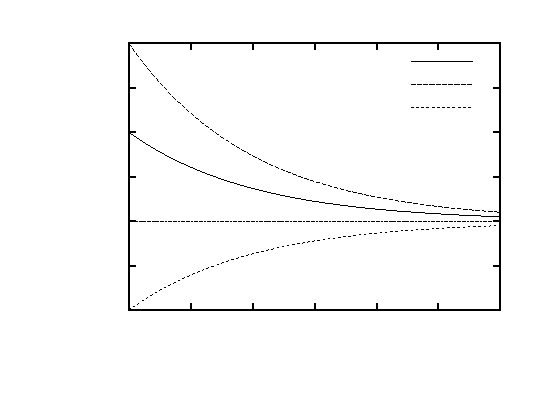
\includegraphics{bucket_v}}%
    \gplfronttext
  \end{picture}%
\endgroup

\end{center}
\end{frame}


\begin{frame}{Variable input}

If the input \crish$i$\cbla changes with time it is often still
possible to solve the equation, but if you have have a multi-neuron
model this might not be possible, so it is often easier to solve
\textsl{numerically}; that is work out the value step by step. We will
look at that but first we should note we have an idea of what happens
from considering the constant case. The solution \textsl{chases} the
input.

\end{frame}
  
\begin{frame}{Variable input}
  Lets look at an example where the input is a sine wave\cblu
  $$i(t)=\sin{t}$$
  \cbla{}and the equation is evolved with \crish$h(0)=0$\cbla{} and three different \crish$\tau$\cbla{}  values.
\end{frame}
  
\begin{frame}{Variable input}
  \vskip -0.7cm
  % GNUPLOT: LaTeX picture with Postscript
\begingroup
  \makeatletter
  \providecommand\color[2][]{%
    \GenericError{(gnuplot) \space\space\space\@spaces}{%
      Package color not loaded in conjunction with
      terminal option `colourtext'%
    }{See the gnuplot documentation for explanation.%
    }{Either use 'blacktext' in gnuplot or load the package
      color.sty in LaTeX.}%
    \renewcommand\color[2][]{}%
  }%
  \providecommand\includegraphics[2][]{%
    \GenericError{(gnuplot) \space\space\space\@spaces}{%
      Package graphicx or graphics not loaded%
    }{See the gnuplot documentation for explanation.%
    }{The gnuplot epslatex terminal needs graphicx.sty or graphics.sty.}%
    \renewcommand\includegraphics[2][]{}%
  }%
  \providecommand\rotatebox[2]{#2}%
  \@ifundefined{ifGPcolor}{%
    \newif\ifGPcolor
    \GPcolorfalse
  }{}%
  \@ifundefined{ifGPblacktext}{%
    \newif\ifGPblacktext
    \GPblacktexttrue
  }{}%
  % define a \g@addto@macro without @ in the name:
  \let\gplgaddtomacro\g@addto@macro
  % define empty templates for all commands taking text:
  \gdef\gplbacktext{}%
  \gdef\gplfronttext{}%
  \makeatother
  \ifGPblacktext
    % no textcolor at all
    \def\colorrgb#1{}%
    \def\colorgray#1{}%
  \else
    % gray or color?
    \ifGPcolor
      \def\colorrgb#1{\color[rgb]{#1}}%
      \def\colorgray#1{\color[gray]{#1}}%
      \expandafter\def\csname LTw\endcsname{\color{white}}%
      \expandafter\def\csname LTb\endcsname{\color{black}}%
      \expandafter\def\csname LTa\endcsname{\color{black}}%
      \expandafter\def\csname LT0\endcsname{\color[rgb]{1,0,0}}%
      \expandafter\def\csname LT1\endcsname{\color[rgb]{0,1,0}}%
      \expandafter\def\csname LT2\endcsname{\color[rgb]{0,0,1}}%
      \expandafter\def\csname LT3\endcsname{\color[rgb]{1,0,1}}%
      \expandafter\def\csname LT4\endcsname{\color[rgb]{0,1,1}}%
      \expandafter\def\csname LT5\endcsname{\color[rgb]{1,1,0}}%
      \expandafter\def\csname LT6\endcsname{\color[rgb]{0,0,0}}%
      \expandafter\def\csname LT7\endcsname{\color[rgb]{1,0.3,0}}%
      \expandafter\def\csname LT8\endcsname{\color[rgb]{0.5,0.5,0.5}}%
    \else
      % gray
      \def\colorrgb#1{\color{black}}%
      \def\colorgray#1{\color[gray]{#1}}%
      \expandafter\def\csname LTw\endcsname{\color{white}}%
      \expandafter\def\csname LTb\endcsname{\color{black}}%
      \expandafter\def\csname LTa\endcsname{\color{black}}%
      \expandafter\def\csname LT0\endcsname{\color{black}}%
      \expandafter\def\csname LT1\endcsname{\color{black}}%
      \expandafter\def\csname LT2\endcsname{\color{black}}%
      \expandafter\def\csname LT3\endcsname{\color{black}}%
      \expandafter\def\csname LT4\endcsname{\color{black}}%
      \expandafter\def\csname LT5\endcsname{\color{black}}%
      \expandafter\def\csname LT6\endcsname{\color{black}}%
      \expandafter\def\csname LT7\endcsname{\color{black}}%
      \expandafter\def\csname LT8\endcsname{\color{black}}%
    \fi
  \fi
  \setlength{\unitlength}{0.0500bp}%
  \begin{picture}(7200.00,5040.00)%
    \gplgaddtomacro\gplbacktext{%
      \csname LTb\endcsname%
      \put(726,440){\makebox(0,0)[r]{\strut{}-1}}%
      \put(726,873){\makebox(0,0)[r]{\strut{}-0.8}}%
      \put(726,1307){\makebox(0,0)[r]{\strut{}-0.6}}%
      \put(726,1740){\makebox(0,0)[r]{\strut{}-0.4}}%
      \put(726,2174){\makebox(0,0)[r]{\strut{}-0.2}}%
      \put(726,2608){\makebox(0,0)[r]{\strut{} 0}}%
      \put(726,3041){\makebox(0,0)[r]{\strut{} 0.2}}%
      \put(726,3475){\makebox(0,0)[r]{\strut{} 0.4}}%
      \put(726,3908){\makebox(0,0)[r]{\strut{} 0.6}}%
      \put(726,4342){\makebox(0,0)[r]{\strut{} 0.8}}%
      \put(726,4775){\makebox(0,0)[r]{\strut{} 1}}%
      \put(858,220){\makebox(0,0){\strut{} 0}}%
      \put(1453,220){\makebox(0,0){\strut{} 2}}%
      \put(2047,220){\makebox(0,0){\strut{} 4}}%
      \put(2642,220){\makebox(0,0){\strut{} 6}}%
      \put(3236,220){\makebox(0,0){\strut{} 8}}%
      \put(3831,220){\makebox(0,0){\strut{} 10}}%
      \put(4425,220){\makebox(0,0){\strut{} 12}}%
      \put(5020,220){\makebox(0,0){\strut{} 14}}%
      \put(5614,220){\makebox(0,0){\strut{} 16}}%
      \put(6209,220){\makebox(0,0){\strut{} 18}}%
      \put(6803,220){\makebox(0,0){\strut{} 20}}%
    }%
    \gplgaddtomacro\gplfronttext{%
      \csname LTb\endcsname%
      \put(5816,4602){\makebox(0,0)[r]{\strut{}$\tau=0.25$}}%
      \csname LTb\endcsname%
      \put(5816,4382){\makebox(0,0)[r]{\strut{}$\tau=2$}}%
      \csname LTb\endcsname%
      \put(5816,4162){\makebox(0,0)[r]{\strut{}$\tau=4$}}%
      \csname LTb\endcsname%
      \put(5816,3942){\makebox(0,0)[r]{\strut{}input}}%
    }%
    \gplbacktext
    \put(0,0){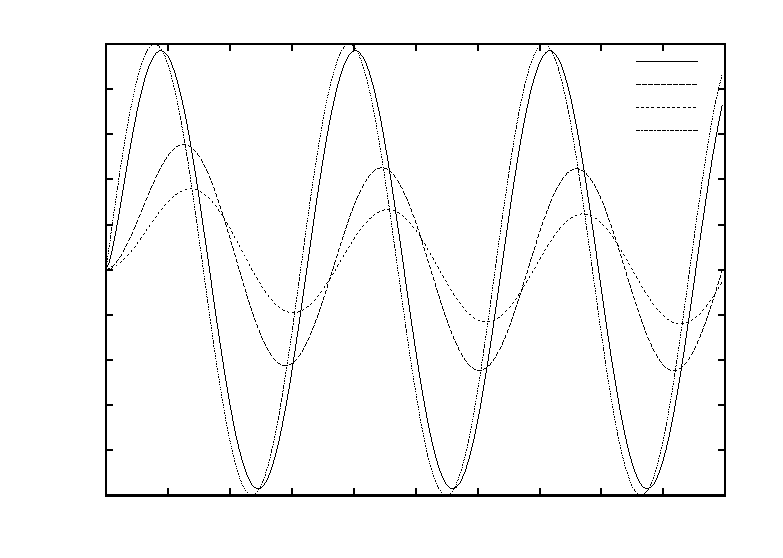
\includegraphics{chasing}}%
    \gplfronttext
  \end{picture}%
\endgroup

\end{frame}

\begin{frame}{Numerical solution}
  \begin{center}
    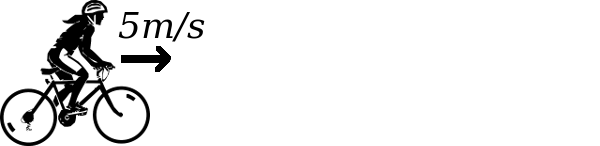
\includegraphics[width=6cm]{cyclist1.png}
  \end{center}
  \end{frame}


\begin{frame}{Numerical solution}
  \begin{center}
    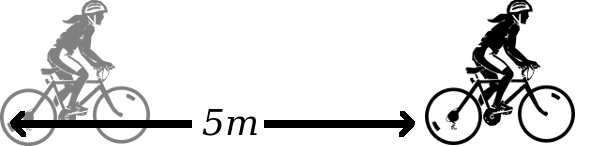
\includegraphics[width=6cm]{cyclist2.png}
  \end{center}
  \end{frame}

\begin{frame}{Numerical solution}
\crish
  $$
\frac{df(t)}{dt}=F(f,t)
$$
\cbla{}This includes our bucket case if we replace \crish$f$\cbla{} with \crish$h$\cbla{} and \crish$F(f,t)$\cbla{}
with \crish$(i-Gh)/C$\cbla.
\end{frame}

\begin{frame}{Eulers approximation}
  \crish
  $$
  f(t+\delta t)\approx f(t)+\delta t F(f,t)
  $$
\cbla
\end{frame}


\begin{frame}{Eulers approximation}
\crish
  $$
t_n=t_0+n\delta t
$$
\cbla
and\crish
$$f(t_n)\approx \cred{}f_n$$
\cbla
  \begin{center}
    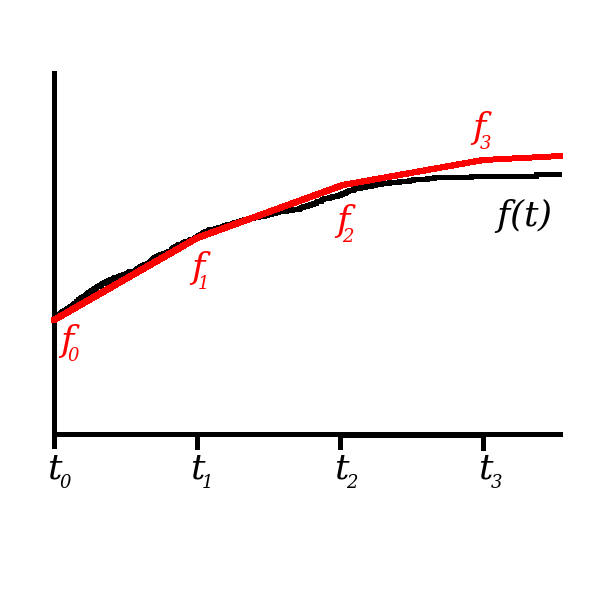
\includegraphics[width=6cm]{f.png}
  \end{center}
\end{frame}

\begin{frame}{Numerical solution}
\crish
$$f_{n+1}=f_n+\delta t F(f_n,t_n)$$
\cbla
  \end{frame}


\begin{frame}{Numerical solution}
\crish
$$
h_{n+1}=\frac{[i(t_n)-Gh_n]\delta t}{C}
$$
\cbla
  \end{frame}

\begin{frame}{Summary}
  \begin{itemize}
  \item Worked out the equation for the height of water in a bucket.
  \item Looked at its solution for constant input.
  \item Gained some intuition as to how it behaves for variable input.
  \item Learned how to solve it numerical using the Euler approximation.
  \end{itemize}
\end{frame}



\end{document}

